%%%%%%%%%%%%%%%%%%%%%%%%%%%%%%%%%%%%%%%%%
% Beamer Presentation
% LaTeX Template
% Version 1.0 (10/11/12)
%
% This template has been downloaded from:
% http://www.LaTeXTemplates.com
%
% License:
% CC BY-NC-SA 3.0 (http://creativecommons.org/licenses/by-nc-sa/3.0/)
%
%%%%%%%%%%%%%%%%%%%%%%%%%%%%%%%%%%%%%%%%%

%----------------------------------------------------------------------------------------
%	PACKAGES AND THEMES
%----------------------------------------------------------------------------------------

\documentclass{beamer}

\mode<presentation> {

% The Beamer class comes with a number of default slide themes
% which change the colors and layouts of slides. Below this is a list
% of all the themes, uncomment each in turn to see what they look like.

%\usetheme{default}
%\usetheme{AnnArbor}
%\usetheme{Antibes}
%\usetheme{Bergen}
%\usetheme{Berkeley}
%\usetheme{Berlin}
%\usetheme{Boadilla}
%\usetheme{CambridgeUS}
%\usetheme{Copenhagen}
%\usetheme{Darmstadt}
%\usetheme{Dresden}
%\usetheme{Frankfurt}
%\usetheme{Goettingen}
%\usetheme{Hannover}
%\usetheme{Ilmenau}
%\usetheme{JuanLesPins}
%\usetheme{Luebeck}
\usetheme{Madrid}
%\usetheme{Malmoe}
%\usetheme{Marburg}
%\usetheme{Montpellier}
%\usetheme{PaloAlto}
%\usetheme{Pittsburgh}
%\usetheme{Rochester}
%\usetheme{Singapore}
%\usetheme{Szeged}
%\usetheme{Warsaw}

% As well as themes, the Beamer class has a number of color themes
% for any slide theme. Uncomment each of these in turn to see how it
% changes the colors of your current slide theme.

%\usecolortheme{albatross}
%\usecolortheme{beaver}
%\usecolortheme{beetle}
%\usecolortheme{crane}
%\usecolortheme{dolphin}
%\usecolortheme{dove}
%\usecolortheme{fly}
%\usecolortheme{lily}
%\usecolortheme{orchid}
%\usecolortheme{rose}
%\usecolortheme{seagull}
%\usecolortheme{seahorse}
%\usecolortheme{whale}
%\usecolortheme{wolverine}

%\setbeamertemplate{footline} % To remove the footer line in all slides uncomment this line
%\setbeamertemplate{footline}[page number] % To replace the footer line in all slides with a simple slide count uncomment this line

%\setbeamertemplate{navigation symbols}{} % To remove the navigation symbols from the bottom of all slides uncomment this line
}
\usepackage{color}
\usepackage{graphicx} % Allows including images
\usepackage{booktabs} % Allows the use of \toprule, \midrule and \bottomrule in tables

%----------------------------------------------------------------------------------------
%	TITLE PAGE
%----------------------------------------------------------------------------------------

\title[STAT 628]{Bodyfat Calculator Development} % The short title appears at the bottom of every slide, the full title is only on the title page
%\author{Ernst C.Wit, Luigi Augugliaro, Hassan Pazira, Javier Gonzalez, Fentaw Abegaz}
\author[Ning Shen, Ruyi Yan, Yiqun Jiang]{} % Your name
\institute[] % Your institution as it will appear on the bottom of every slide, may be shorthand to save space
{
Ning Shen, Ruyi Yan, Yiqun Jiang \\ % Your institution for the title page
\medskip
%\textit{john@smith.com} % Your email address
}
\date{Jan 7, 2019} % Date, can be changed to a custom date


\begin{document}

\begin{frame}
\titlepage % Print the title page as the first slide
\end{frame}

\begin{frame}
\frametitle{Overview} % Table of contents slide, comment this block out to remove it
\tableofcontents % Throughout your presentation, if you choose to use \section{} and \subsection{} commands, these will automatically be printed on this slide as an overview of your presentation
\end{frame}

%----------------------------------------------------------------------------------------
%	PRESENTATION SLIDES
%----------------------------------------------------------------------------------------

%------------------------------------------------
\section{Introduction} % Sections can be created in order to organize your presentation into discrete blocks, all sections and subsections are automatically printed in the table of contents as an overview of the talk

%\subsection{Subsection Example} % A subsection can be created just before a set of slides with a common theme to further break down your presentation into chunks

\section{Background \& Motivation}
\section{Data Cleaning}
\section{Statistical Analysis}
\section{Model Summary}
\section{Diagnostics}
\section{Strength \& Weakness} 
%------------------------------------------------

\begin{frame}
\frametitle{Introduction}
In this project, we explores what factors effect body fat, furthermore, expect to develop a reliable but simple calculator for body fat.\\~\\  We focus on body fat data file containing only 252 males' bodyfat, density, ages, weights, heights  and some body part circumferences trying to extract useful information for our body fat calculator.\\~\\  Here, to achieve our goal of simplicity, we just used linear regression model. Linear regression model is an easily understandable model with parameters not hard to interpret. Besides, it is also enough flexible as we could add interaction terms to explain the relationship between different variables.
\end{frame}


%-----------------------------------------------

\begin{frame}
\frametitle{Background \& Motivation}
\begin{itemize}
\item Importance of body fat for evaluating obesity.\\~\\
\item Extant estimation methods--troublesome/costly\\~\\
\item Aim to develop a simple and reliable calculator
\end{itemize}
\end{frame}

%------------------------------------------------

\begin{frame}
\frametitle{Data Cleaning}
\begin{itemize}
\item boxplots or histograms--find extreme values. \\~\\
\item variable relationship--find influential points. \\~\\
\end{itemize}
\end{frame}
%------------------------------------------------
\begin{frame}
\frametitle{Data Cleaning: Histograms}
\begin{itemize}
\begin{figure}
\centering
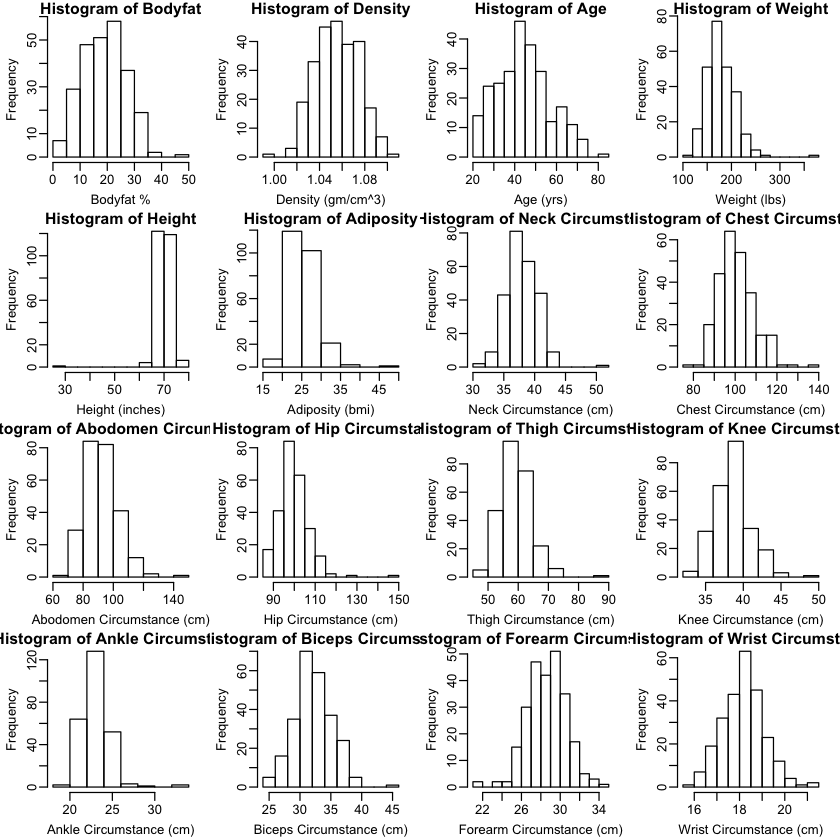
\includegraphics[height=8cm,width=10cm]{histograms.png}
\caption{histogram.png}
\label{2}
\end{figure}
\end{itemize}
\end{frame}
%-----------------------------------------

\begin{frame}
\frametitle{Data Cleaning: Deal with Extreme Data Points}
\begin{itemize}
\item No.182 obs.: extreme value 0 of body fat, which make no sense--delete\\~\\ 
\item No.42 obs.: extreme value 29.5 of height, but we check other variables of the observation and define the height is a typo--recompute the height using BMI equation. \\~\\
\item No.216 obs.: extreme value 0.995 of density, however, all other variables of the obs seems reasonable--keep it. \\~\\
\item No.39 obs.: extreme value for weight, adiposity and most body part circumference. We infer that it is a fat person--keep it.
\end{itemize}
\end{frame}
%------------------------------------------------

\begin{frame}
\frametitle{Data Cleaning: Check Influential Points}

\begin{block}{BMI vs. calculated BMI Plot and Bodyfat vs. Density Plot}

\begin{figure}
\begin{minipage}[t]{0.5\linewidth}
\centering
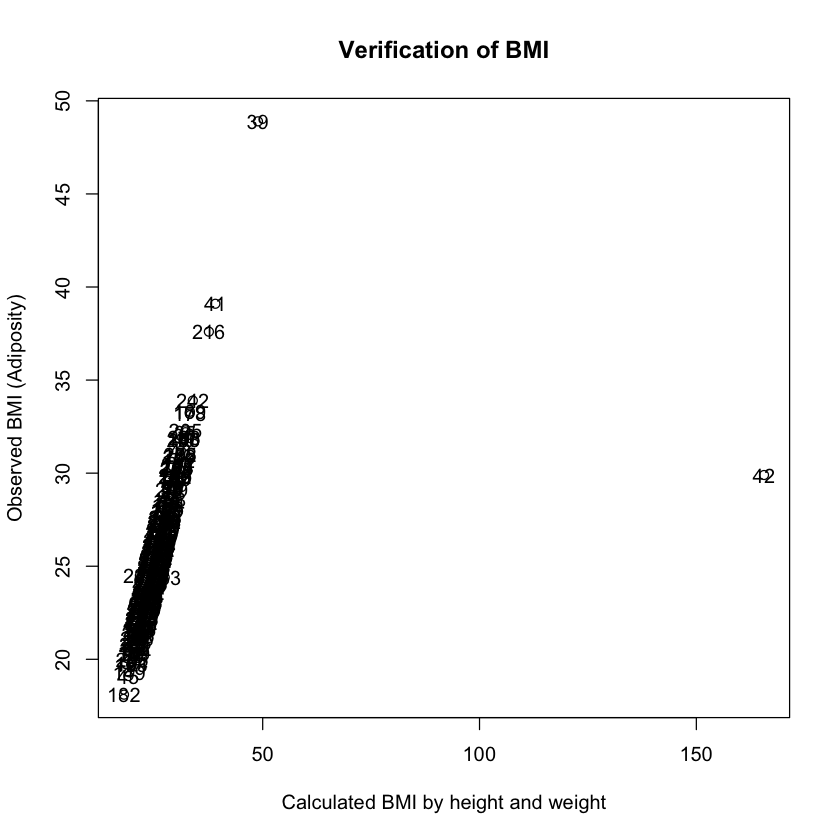
\includegraphics[width=2.2in]{pic1.png}
\caption{BMI vs. calculated BMI Plot}
\label{fig:side:a}
\end{minipage}%
\begin{minipage}[t]{0.5\linewidth}
\centering
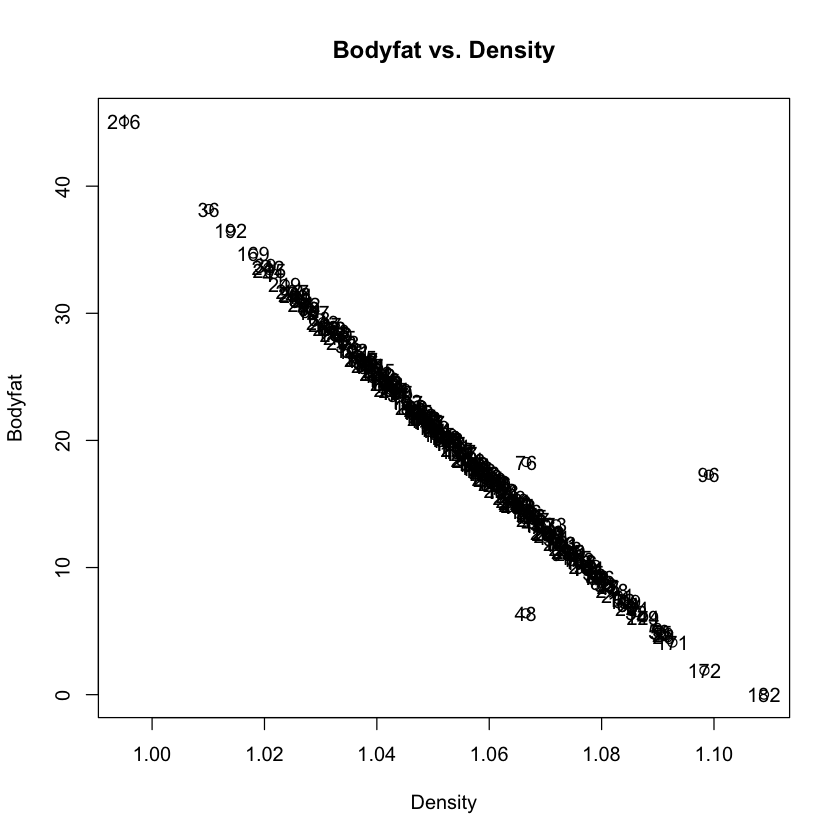
\includegraphics[width=2.2in]{pic2}
\caption{Bodyfat vs. Density Plot}
\label{fig:side:b}
\end{minipage}
\end{figure}

\end{block}
\end{frame}
%-----------------------------------------

\begin{frame}
\frametitle{Data Cleaning: Deal with Influential Data Points}
\begin{itemize}
\item In this data set, two clear relationships between variabales are: \\
1) linear relationship between density and body fat, \\
2) BMI equation defined relationship between weight, height and adiposity. \\
- We check the relationships to find influential points here.
\item No.48,96 are considered as influential points due to the Cook's distance plot. Since we are not sure where the error came from, we decided to simply remove these 2 samples.
\end{itemize}
\end{frame}
%------------------------------------------------



\begin{frame}
\frametitle{Statistical Analysis}
\begin{itemize}
\item Below are scatterplots between bodyfat and predictors. Except for age and height, other variables all seem to have somewhat linear relationship with bodyfat. \\~\\
\end{itemize}
\end{frame}
%------------------------------------------------


\begin{frame}
\frametitle{Statistical Analysis: Scatterplots}
\begin{itemize}

\begin{figure}
\centering
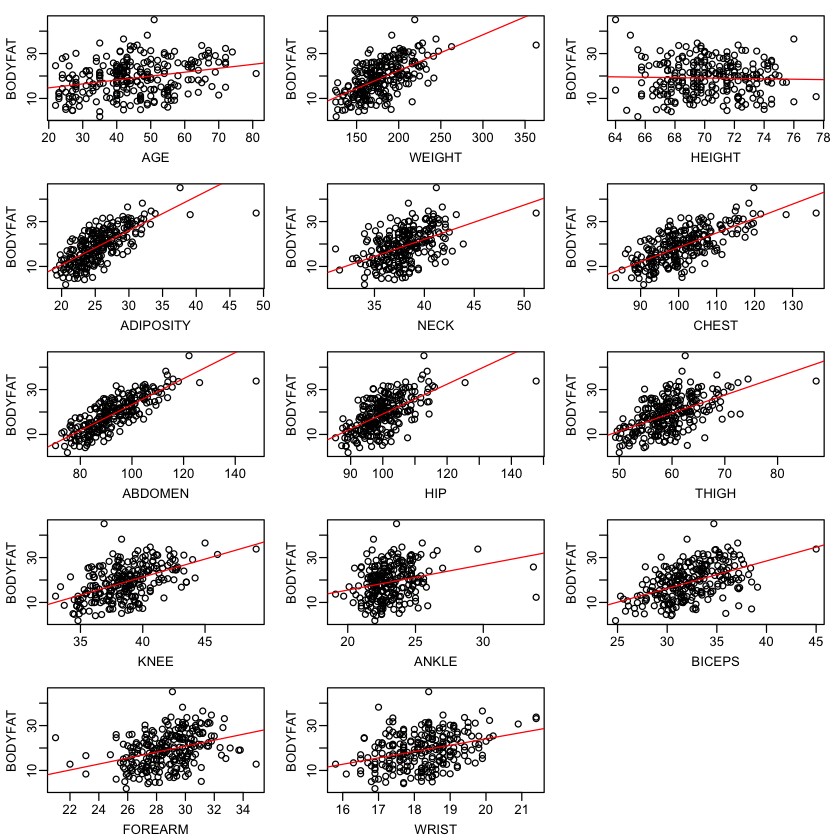
\includegraphics[height=7cm,width=10cm]{Scatterplot.png}
\label{2}
\end{figure}
\end{itemize}
\end{frame}
%------------------------------------------------

\begin{frame}
\frametitle{Statistical Analysis: Scatterplots}
\begin{itemize}
\begin{figure}
\centering
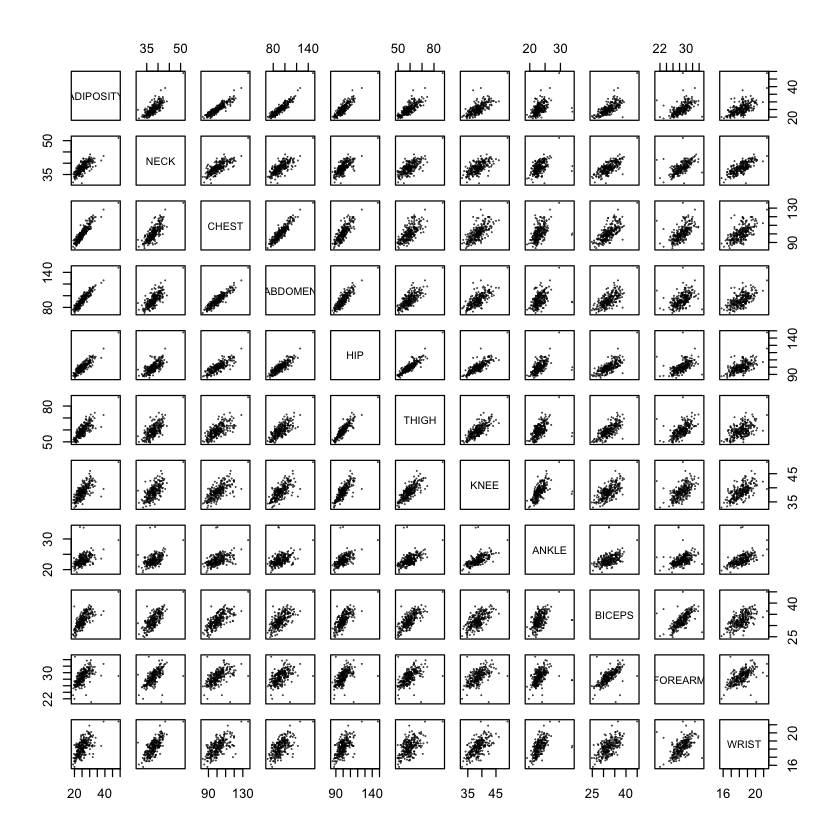
\includegraphics[height=8cm,width=10cm]{pairsplot.png}
\label{2}
\end{figure}
\end{itemize}
\end{frame}
%------------------------------------------------
\begin{frame}
\frametitle{Statistical Analysis}

\begin{block}{Model0}
$$B(\%) = \beta_1*W (lbs) + \beta_0,$$
where B is the bodyfat percentage (unit: $\%$), and W is the weight (unit: pound).
\end{block}
\begin{itemize}
    \item $R^2$=0.369
    \item   Summary statistics of the model:
            \begin{table}
	        \centering
        	\begin{tabular}{cccc}  
	        	\toprule
	        	& Estimate &	Std. Error &		Pr(\textgreater\abs{t})\\  
	        	\midrule        %画一条横线
	        	(Intercept) &	-9.60 &	2.400  &	9.6e-05 \\
	        	 WEIGHT &	0.16 &	0.013 &		1.6e-26 \\
	        	\bottomrule
        	\end{tabular}
        \end{table}
\end{itemize}









\end{frame}
%------------------------------------------------

\begin{frame}
\frametitle{Statistical Analysis}
\begin{block}{Add One Variable}

Then we want to add on just one of body part circumference variables in order to increase the R-squared but keep the simplicity of our model. And 'abdomen' seems to be the best choice.
\end{block}

\begin{center}
\textbf{Table 1}~~$R^2$ table\\

\begin{tabular}{ccccc} \toprule
NECK &	CHEST &	ABDOMEN &	HIP &	THIGH \\ 
\hline
0.37 &	0.487 &	0.713 &	0.388 &	0.371 \\
\bottomrule
\end{tabular}

\begin{tabular}{cccccccccc} \toprule
	KNEE &	ANKLE &	BICEPS &	FOREARM	& WRIST \\ 
\hline
	0.37 &	0.392 &	0.369 &	0.37 &	0.389 \\
\bottomrule
\end{tabular}

\end{center}


\end{frame}

%------------------------------------------------
\begin{frame}
\frametitle{Statistical Analysis}
\begin{block}{Model1}
$$B(\%) = \beta_2*A (cm) + \beta_1*W (lbs) + \beta_0,$$
where B is the bodyfat percentage (unit: $\%$), A is the abdomen circumference (unit: centimeter), and W is the weight (unit: pound).
\end{block}
\begin{itemize}
    \item $R^2$=0.713
    \item   Summary statistics of the model:
            \begin{table}
	        \centering
        	\begin{tabular}{ccc}  
	        	\toprule
	        	& Estimate &	Pr(\textgreater\abs{t})\\  
	        	\midrule        %画一条横线
	        	 (Intercept) &	-41.00 &	2.7e-42 \\
	        	 WEIGHT &	-0.14 &	2.5e-11 \\
		         ABDOMEN &	0.91 &	6.0e-44 \\
	        	\bottomrule
        	\end{tabular}
        \end{table}
\end{itemize}
\end{frame}
%------------------------------------------------
\begin{frame}
\frametitle{Statistical Analysis}
\begin{block}{Model2}
$$B(\%) = \beta_3*A*W + \beta_2*A (cm) + \beta_1*W (lbs) + \beta_0,$$

\end{block}
\begin{itemize}
    \item $R^2$=0.724
    \item   Summary statistics of the model:
            \begin{table}
	        \centering
        	\begin{tabular}{ccc}  
	        	\toprule
	        	& Estimate &	Pr(\textgreater\abs{t})\\  
	        	\midrule        %画一条横线
	        	 (Intercept) &	-64.0000 &	8.5e-15 \\
	        	 WEIGHT &	-0.0031 &	9.5e-01 \\
		         ABDOMEN &	1.1000 &	4.1e-29 \\
		         WEIGHT:ABDOMEN &	-0.0013 &	1.7e-03 \\
	        	\bottomrule
        	\end{tabular}
        \end{table}
\end{itemize}
\end{frame}
%------------------------------------------------


\begin{frame}
\frametitle{Statistical Analysis}

\begin{block}{Residual Plot and Cook's Distance Plot}

\begin{figure}
\begin{minipage}[t]{0.5\linewidth}
\centering
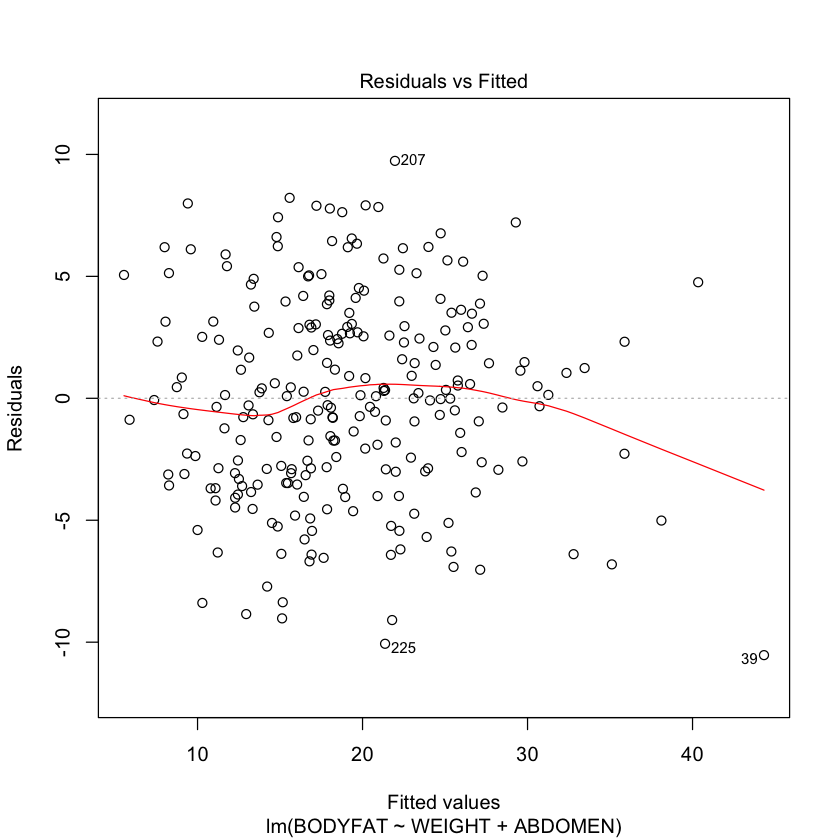
\includegraphics[width=2.2in]{residualplot.png}
\caption{Residual Plot}
\label{fig:side:a}
\end{minipage}%
\begin{minipage}[t]{0.5\linewidth}
\centering
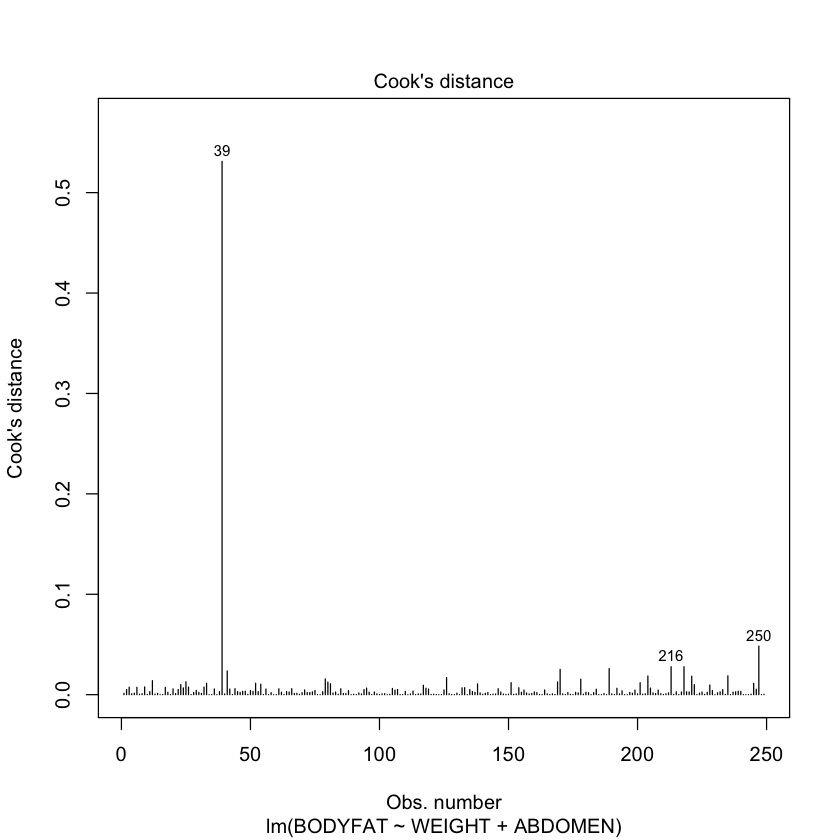
\includegraphics[width=2.2in]{cookplot}
\caption{Cook's Distance}
\label{fig:side:b}
\end{minipage}
\end{figure}

\end{block}
\end{frame}

%------------------------------------------------
\begin{frame}
\frametitle{Statistical Analysis} 
\begin{itemize}
    \item After deleting No.39 sample:\\
    - $R^2$=0.718\\
    - Summary statistics of the model:
            \begin{table}
	        \centering
        	\begin{tabular}{cccc}  
	        	\toprule
	        	& Estimate &	Std. Error & Pr(\textgreater\abs{t})\\  
	        	\midrule        %画一条横线
	        	 (Intercept) &	-42.00 &	2.500 &	9.7e-44 \\
	           	WEIGHT &	-0.12 &	0.020 &	3.2e-09 \\
		         ABDOMEN &	0.90 &	0.052 &	5.5e-44 \\
	        	\bottomrule
        	\end{tabular}
        \end{table}
\end{itemize}


\end{frame}


%------------------------------------------------------------------

\begin{frame}{Statistical Analysis}
\begin{itemize}
    \item We want to explore the possibility of more than two predictors, we try to add on one body part circumference variables other than ABDOMEN to the current model and check out the R-squared with different additional variables.
    \item  R-square table:
        \begin{center}
        \begin{tabular}{ccccc}\toprule
        NECK &	CHEST &	HIP &	THIGH &	KNEE \\
        \hline
        0.723 &	0.719 &	0.718 &	0.722 &	0.718 \\
        \bottomrule
        \end{tabular}
        
        \begin{tabular}{ccccc}\toprule
         ANKLE &	BICEPS & FOREARM &	WRIST\\
        \hline
        0.718 &	0.72 &	0.719 &	0.73\\
        \bottomrule
        \end{tabular}

        \end{center}
       

    \item Although adding on WRIST can increase the $R^2$ maximumly, the increment is negligible (0.73 - 0.718 = 0.012).
\end{itemize}

\end{frame}
%------------------------------------------------

\begin{frame}
\frametitle{Statistical Analysis}

\textbf{The final model is:}
$$B(\%) = 0.90*A (cm) - 0.12*W (lbs) - 42,$$
 where B is the bodyfat percentage (unit is $\%$), A is the abdomen circumference (unit: centimeter), and W is the weight (unit: pound).


\end{frame}

%------------------------------------------------
%-------------------------------------------------
\begin{frame}
\frametitle{Diagnostics}
\begin{itemize}
	\item Residual plot, QQ-plot and Cook's distance Plot:
	\begin{figure}
		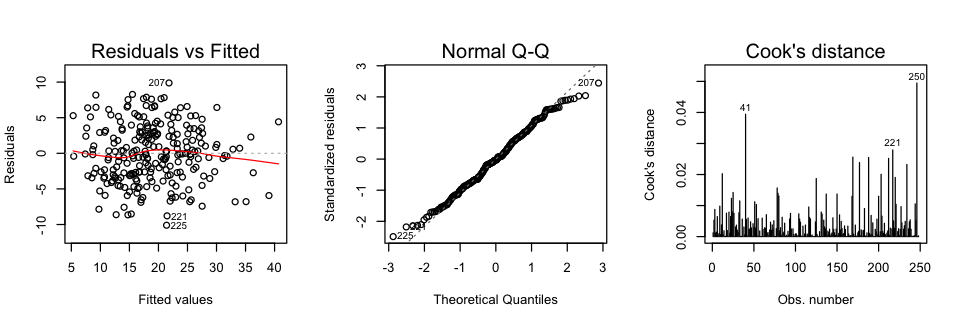
\includegraphics[width=1\linewidth]{Diagnostics.png}
	\end{figure}
\end{itemize}
\end{frame}



%-------------------------------------------------

\begin{frame}
\frametitle{Model Summary}
\begin{itemize}
	\item $R^2 = 0.718; \text{Adjusted}\ R^2 = 0.716$
	
	\item Summary statistics of the model:
	\begin{table}
		\centering
		\begin{tabular}{cccc}   %三个c是因为三列,令每列显示在中间显示,也可以是l或r
			\toprule
			& Estimate &	Std. Error	&  P-Value\\  
			\midrule        %画一条横线
			 (Intercept) & -42.00  & 2.500  & 9.7e-44 \\
			 WEIGHT & -0.12	  & 0.020  & 3.2e-09 \\
			 ABDOMEN & 0.90  & 0.052  & 5.5e-44 \\
			\bottomrule
		\end{tabular}
	\end{table}

	\item Confidence intervals:
	\begin{table}
		\centering
		\begin{tabular}{ccc}   %三个c是因为三列,令每列显示在中间显示,也可以是l或r
			\toprule
			& 2.5\% &	97.5\% \\  
			\midrule        %画一条横线
			(Intercept) & -47.12 &	-37.40 \\
			WEIGHT & -0.16 &	-0.08 \\
			ABDOMEN & 0.79  &	1.00\\
			\bottomrule
		\end{tabular}
	\end{table}

\end{itemize}
\end{frame}

%-------------------------------------------------

\begin{frame}
\frametitle{Interpretation}
\begin{itemize}
	\item \textbf{Possible rule of thumb:} 9/10 abdomen circumference minus 1/8 weight, and minus 42.
	\item \textbf{Example Usage:} 
		\begin{table}
		\centering
		\begin{tabular}{cccc}   %三个c是因为三列,令每列显示在中间显示,也可以是l或r
			\toprule
			Abdomen & Weight &	Est.Bodyfat	& Appr.Est.Bodyfat\\  
			\midrule        %画一条横线
			80 cm & 150 lbs & 11.4\% & 11.25\% \\
			90 cm & 150 lbs & 21.3\% & 20.25\% \\
			\bottomrule
		\end{tabular}
	\end{table}
	
	\item \textbf{Inference about Relationship:} Linear relationship clearly exists between the response variable and predictors ($P = 4.78e^{-68}$). Variation explained by this model achieved more than 70\%.
	
\end{itemize}
\end{frame}


%------------------------------------------------------------
\begin{frame}
\frametitle{Strength and Weakness}
\begin{itemize}
	\item \textbf{strength:}\\
	- Simplicity.\\
	- Assumption verification.\\
	- Explanation of variation.
	\item \textbf{Weakness:}\\
	- Small sample size.\\
	- Narrow scope of application.\\
	- Colinearity.\\
	- Further complex models haven't been tried.\\
	- This model doesn't make sure predicted bodyfat is positive!
	

\end{itemize}
\end{frame}

%-------------------------------------------------------------
\begin{frame}
\Huge{\centerline{Thank you}}
\end{frame}



\end{document}
